\newpage
\texHeader

% The second reference type is a simple which
can be spotted in the next ``Node'' class. It's represented by just the arrow. EReferences name are immediately followed by their multiplicity % Include a reference to UML here if they need a refresher?
and then, just like an attribute, a colon and datatype.

While we're on the topic of syntax, lets have a quick overview on MOSL operators. The \texttt{`@'} before a name represents a bounded variable, \texttt{`--'} shows intended removal, and the opposite \texttt{`++'} operator signals something to be created. The destruction and creation operators can be placed before names or other operators, such as references.  All black items are elements of context, and must exist before and after the control flow. 

Lets go back to looking at the code. In the ``Node'' class, a few methods have been declared. You can see each function is remarkably small. In fact,the only thing the functions are doing are calling patterns. These patterns represent dynamic action within the program. Overall, the method and return statements are used just for control flow. A common format in a method like this would be {\texttt if (this) [pattern] else [pattern] }. The activities are never directly implemented. But where are these pattern files defined?

After many long discussions on correct control flow, it was decided that patterns must follow a strict, predictable path. Inspect Figure~\ref{fig_modelSpecification} again, and observe the locations where the patterns are stored. You'll notice that there is a folder for the ``Node'' class, and a folder for each method within that space. There's no folder for ``List'' purely because it never calls a pattern. It is imperative in the future that every pattern created follows this `Class/Method/patternName.pattern' set up. % Expand on this?? Seems to cut short

On a final note, one of the really neat things about references in MOSL is that the other object involved in the reference is automatically updated! Check out the ``DeleteNode'' pattern (Fig ~\ref{fig_MOSLOverview}). 

 \begin{figure}[htbp]
  \centering
  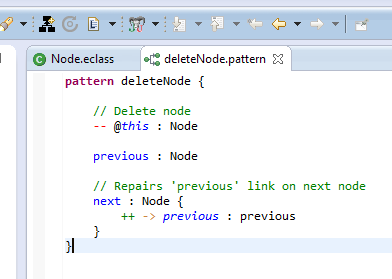
\includegraphics[width=0.6\textwidth]{MOSL_finalSyntaxReview}
  \caption{Eclipse/Ecore: The ``DeleteNode'' Pattern}
  \label{fig_MOSLOverview}
\end{figure}

